\documentclass[letterpaper,12pt]{article}
\usepackage{array}
\usepackage{threeparttable}
\usepackage{geometry}
\geometry{letterpaper,tmargin=1in,bmargin=1in,lmargin=1.25in,rmargin=1.25in}
\usepackage{fancyhdr,lastpage}
\pagestyle{fancy}
\lhead{}
\chead{}
\rhead{}
\lfoot{}
\cfoot{}
\rfoot{\footnotesize\textsl{Page \thepage\ of \pageref{LastPage}}}
\renewcommand\headrulewidth{0pt}
\renewcommand\footrulewidth{0pt}
\usepackage[format=hang,font=normalsize,labelfont=bf]{caption}
\usepackage{listings}
\lstset{frame=single,
  language=Python,
  showstringspaces=false,
  columns=flexible,
  basicstyle={\small\ttfamily},
  numbers=none,
  breaklines=true,
  breakatwhitespace=true
  tabsize=3
}
\usepackage{amsmath}
\usepackage{amssymb}
\usepackage{amsthm}

\usepackage{mathrsfs}

\usepackage{harvard}
\usepackage{setspace}
\usepackage{float,color}
\usepackage[pdftex]{graphicx}
\usepackage{hyperref}

\hypersetup{colorlinks,linkcolor=red,urlcolor=blue}
\theoremstyle{definition}
\newtheorem{theorem}{Theorem}
\newtheorem{acknowledgement}[theorem]{Acknowledgement}
\newtheorem{algorithm}[theorem]{Algorithm}
\newtheorem{axiom}[theorem]{Axiom}
\newtheorem{case}[theorem]{Case}
\newtheorem{claim}[theorem]{Claim}
\newtheorem{conclusion}[theorem]{Conclusion}
\newtheorem{condition}[theorem]{Condition}
\newtheorem{conjecture}[theorem]{Conjecture}
\newtheorem{corollary}[theorem]{Corollary}
\newtheorem{criterion}[theorem]{Criterion}
\newtheorem{definition}[theorem]{Definition}
\newtheorem{derivation}{Derivation} % Number derivations on their own
\newtheorem{example}[theorem]{Example}
\newtheorem{exercise}[theorem]{Exercise}
\newtheorem{lemma}[theorem]{Lemma}
\newtheorem{notation}[theorem]{Notation}
\newtheorem{problem}[theorem]{Problem}
\newtheorem{proposition}{Proposition} % Number propositions on their own
\newtheorem{remark}[theorem]{Remark}
\newtheorem{solution}[theorem]{Solution}
\newtheorem{summary}[theorem]{Summary}
%\numberwithin{equation}{section}
\bibliographystyle{aer}
\newcommand\ve{\varepsilon}
\newcommand\boldline{\arrayrulewidth{1pt}\hline}

\usepackage{mathtools}
% commands
\DeclarePairedDelimiterX{\inp}[2]{\langle}{\rangle}{#1, #2}
\newcommand{\norm}[1]{\left\lVert#1\right\rVert}
\usepackage{mathrsfs}

\setcounter{MaxMatrixCols}{20}
\graphicspath{{.}}
\begin{document}

\begin{flushleft}
  \textbf{\large{Problem Set \#5, Linear Programming}} \\
  OSM Lab: Math \\
  Rebekah Dix
\end{flushleft}

\vspace{5mm}
See the Jupyter notebook for problems not solved here.
\subsection*{Exercises 1-4: See Jupyter Notebook}
\subsection*{Exercise 5}
\subsubsection*{Part (i)}
The dictionaries after each pivot are:
\begin{equation*}
\begin{matrix}
\zeta &= & & & 3x_1 &+& x_2 \\
\hline
w_1 &= &15 &-& x_1 &-& 3x_2\\
w_2 &= &18 &-& 2x_1 &-& 3x_2 \\
w_3 &= &4 &- & x_1 &+& x_2
\end{matrix}
\end{equation*}

\begin{equation*}
\begin{matrix}
\zeta &= &12&-& 3w_3 &+& 4x_2 \\
\hline
w_1 &= &11 &+& w_3 &-& 4x_2\\
w_2 &= &10 &+& 2w_3 &-& 5x_2 \\
x_1 &= &4 &- & w_3 &+& x_2
\end{matrix}
\end{equation*}

\begin{equation*}
\begin{matrix}
\zeta &= &20&-& \frac{7}{5} w_3 &-& \frac{4}{5} w_2 \\
\hline
w_1 &= &3 &-& \frac{3}{5} w_3 &+& \frac{4}{5}w_2 \\
x_2 &= &2&+& \frac{2}{5} w_3 &-& \frac{1}{5} w_2 \\
x_1 &= &6&- & \frac{3}{5} w_3 &-& \frac{1}{5} w_2
\end{matrix}
\end{equation*}
Therefore, the optimum is $(6,2)$ and the optimum is $20$, which is what we found through brute force. 

\subsubsection*{Part (ii)}
The dictionaries after each pivot are:
\begin{equation*}
\begin{matrix}
\zeta &= & & & 4x &+& 6y \\
\hline
w_1 &= &11 &+& x &-& y\\
w_2 &= &27 &-& x &-& y \\
w_3 &= &90 &- & 2x &-& 5y
\end{matrix}
\end{equation*}

\begin{equation*}
\begin{matrix}
\zeta &= &108 &-& 4w_2 &+& 2y \\
\hline
w_1 &= &38 &-& w_2 &-&2y\\
x &= &27 &-& w_2 &-& y \\
w_3 &= &36 &+ & 2w_2 &-& 3y
\end{matrix}
\end{equation*}

\begin{equation*}
\begin{matrix}
\zeta &= &132 &-& \frac{8}{3} w_2 &-& \frac{2}{3} w_3 \\
\hline
w_1 &= &14 &-& \frac{7}{3} w_2 &+& \frac{2}{3}w_3 \\
x &= &15 &-& \frac{5}{2} w_2 &-& \frac{1}{3} w_3 \\
y &= &12 &-& \frac{2}{3}w_2 &-& \frac{1}{3}w_3 \\
\end{matrix}
\end{equation*}
Thus, the optimizer is $(x,y) = (15,12)$, which is what we found through brute force. The optimum value is $132$. 

\subsection*{Exercise 6}
The dictionaries after each pivot are:
\begin{equation*}
\begin{matrix}
\zeta &= & & & 4x_1 &+& 3x_2 \\
\hline
w_1 &= &150 &-& x_1 &-& x_2\\
w_2 &= &360 &-& 3x_1 &-& 2x_2 \\
w_3 &= &200&- & x_2 & &
\end{matrix}
\end{equation*}

\begin{equation*}
\begin{matrix}
\zeta &= &450&-& 3w_1 &+& x_1 \\
\hline
x_2 &= &150&-& w_1 &-&x_1\\
w_2 &= &60 &-& x_1 &+&2w_1\\
w_3 &= &50 &- & w_1 &+& x_1
\end{matrix}
\end{equation*}

\begin{equation*}
\begin{matrix}
\zeta &= &510&-& w_1 &-& w_2 \\
\hline
x_2 &= &90&-& 3w_1 &+&w_2\\
x_1 &= &60 &-& w_2 &+&2w_1\\
w_3 &= &110 &+& w_1 &-& w_2
\end{matrix}
\end{equation*}

The optimizer is $(60,90)$ and the optimum is $510$. 

\subsection*{Exercise 7}
\subsubsection*{Part (i)}
We first setup the auxiliary problem. The dictionaries after each pivot are:
\begin{equation*}
\begin{matrix}
\zeta &= & & & & & &- & x_0 \\
\hline
x_3 &=& -8 &+& 4x_1 &+&2x_2 &+&x_0 \\
x_4 &=& 6 &+&2x_1 &-&3x_2 &+&x_0 \\
x_5 &=& 3 &-& x_1 & & &+& x_0
\end{matrix}
\end{equation*}

\begin{equation*}
\begin{matrix}
\zeta &=&-8&-&x_3&+&x_1& +& 2x_2 \\
\hline
x_0&=& 8 &+& x_3 &-&4x_1 &-&2x_2 \\
x_4 &=& 14 &-&2x_1 &-&5x_2 &+&x_3 \\
x_5 &=&11 &-& 5x_1 &-&2x_2&+& x_3
\end{matrix}
\end{equation*}

\begin{equation*}
\begin{matrix}
\zeta &= & & & & & &- & x_0 \\
\hline
x_1 &=& 2 &+& \frac{1}{4} x_3 &-& \frac{1}{2} x_2 &-& \frac{1}{4}x_0 \\
x_4 &=& 10 &+& \frac{1}{2}x_0 &-&4x_2 &+&\frac{1}{2} x_3 \\
x_5 &=&1 &+& \frac{5}{4}x_0 &+& \frac{1}{2}x_2 &-& \frac{1}{4} x_3
\end{matrix}
\end{equation*}

Now we can use the original problem with a different starting point: 
\begin{equation*}
\begin{matrix}
\zeta &=&2 &+& \frac{3}{2} x_2 & +& \frac{1}{4}x_3 \\
\hline
x_1 &=& 2 &+& \frac{1}{4} x_3 &-& \frac{1}{2} x_2\\
x_4 &=& 10 &-&4x_2 &+&\frac{1}{2} x_3 \\
x_5 &=&1 &+& \frac{1}{2}x_2 &-& \frac{1}{4} x_3
\end{matrix}
\end{equation*}

\begin{equation*}
\begin{matrix}
\zeta &=&3 &+& 2x_2 &-& x_5 \\
\hline
x_1 &=& 3 &-&x_5 & &\\
x_4 &=& 12 &-&3x_2 &-&2x_5 \\
x_3 &=&4 &+& 2x_2 &-& 4x_5
\end{matrix}
\end{equation*}

\begin{equation*}
\begin{matrix}
\zeta &=&11&-& \frac{2}{3} x_4 &-& \frac{7}{3} x_5 \\
\hline
x_1 &=& 3 &-&x_5 & &\\
x_2 &=& 4 &-& \frac{1}{4} x_4 &-& \frac{2}{3} x_5 \\
x_3 &=& 12 &-& \frac{2}{3} x_4 &-& \frac{16}{3} x_5
\end{matrix}
\end{equation*}

The optimizer is $(3,4)$ and the optimum is $11$.

\subsubsection*{Part (ii)}
We first setup the auxiliary problem:
\begin{equation}
\begin{matrix}
    \zeta & = & & & & & & - & x_0 \\
    \hline
    x_3 & = & 15 & - & 5x_1 & - & 3x_2 & + & x_0 \\
    x_4 & = & 15 & - & 3x_1 & - & 5x_2 & + & x_0 \\
    x_5 & = & -12 & - & 4x_1 & + & 3x_2 & + & x_0 \\
\end{matrix}
\end{equation}
\begin{equation}
\begin{matrix}
 \zeta & = &  -12 & - & 4x_1 & + & 3x_2 & - & x_5 \\
    \hline
    x_3 & = & 27 & - & x_1 & - & 6x_2 & + & x_5 \\
    x_4 & = & 27 & + & x_1 & - & 8x_2 & + & x_5 \\
    x_0 & = & 12 & + & 4x_1 & - & 3x_2 & + & x_5 \\
\end{matrix}
\end{equation}
\begin{equation}
\begin{matrix}
\zeta & = & -\tfrac{15}{8} & - & \tfrac{29}{8}x_1 & - & \tfrac{3}{8}x_4 & - & \tfrac{5}{8}x_5 \\
    \hline
    x_3 & = & \tfrac{27}{4} & - & \tfrac{7}{4}x_1 & + & \tfrac{3}{4}x_4 & + & \tfrac{1}{4}x_5 \\
    x_2 & = & \tfrac{27}{8} & + & \tfrac{1}{8}x_1 & - & \tfrac{1}{8}x_4 & + & \tfrac{1}{8}x_5 \\
    x_0 & = & \tfrac{15}{8} & + & \tfrac{29}{8}x_1 & + & \tfrac{3}{8}x_4 & + & \tfrac{5}{8}x_5 \\
\end{matrix}
\end{equation}

All variables decrease the optimum. Therefore, 0 is not the optimum in the auxiliary problem. Thus, the original problem has no feasible solutions. 

\subsubsection*{Part (iii)}
The dictionaries after each pivot are:
\begin{equation}
\begin{matrix}
\zeta & = & & - & 3x_1 & + & x_2 \\
    \hline
    x_3 & = & 4 & & & - & x_2 \\
    x_4 & = & 6 & + & 2x_1 & - & 3x_2 \\
\end{matrix}
\end{equation}

\begin{equation}
\begin{matrix}
    \zeta & = & 2 & - & \tfrac{7}{3}x_1 & - & \tfrac{1}{3}x_4 \\
    \hline
    x_3 & = & 2 & - & \tfrac{2}{3}x_1 & + & \tfrac{1}{3}x_4 \\
    x_2 & = & 2 & + & \tfrac{2}{3}x_1 & - &
    \tfrac{1}{3}x_4 \\
\end{matrix}
\end{equation}
Therefore the optimizer is $(0,2)$ and the optimum is 2.

\subsubsection*{Exercise 8.8} [[Thanks Matt for the help with this example]].
Consider the following linear program:
\begin{align*}
  &\text{maximize} \ \ -x - y - z \\
  &\text{subject to} \ \ -x + y \leq 1 \\
  &\qquad \qquad \ \ \ x - y \leq 1 \\
  &\qquad \qquad \ \ \ x - z \leq 1 \\
  &\qquad \qquad \ \ \ -x + z \leq 1 \\
  &\qquad \qquad \ \ \ x , y, z \geq 0
\end{align*}
\begin{figure}[H]
  \centering
	\begin{center}
		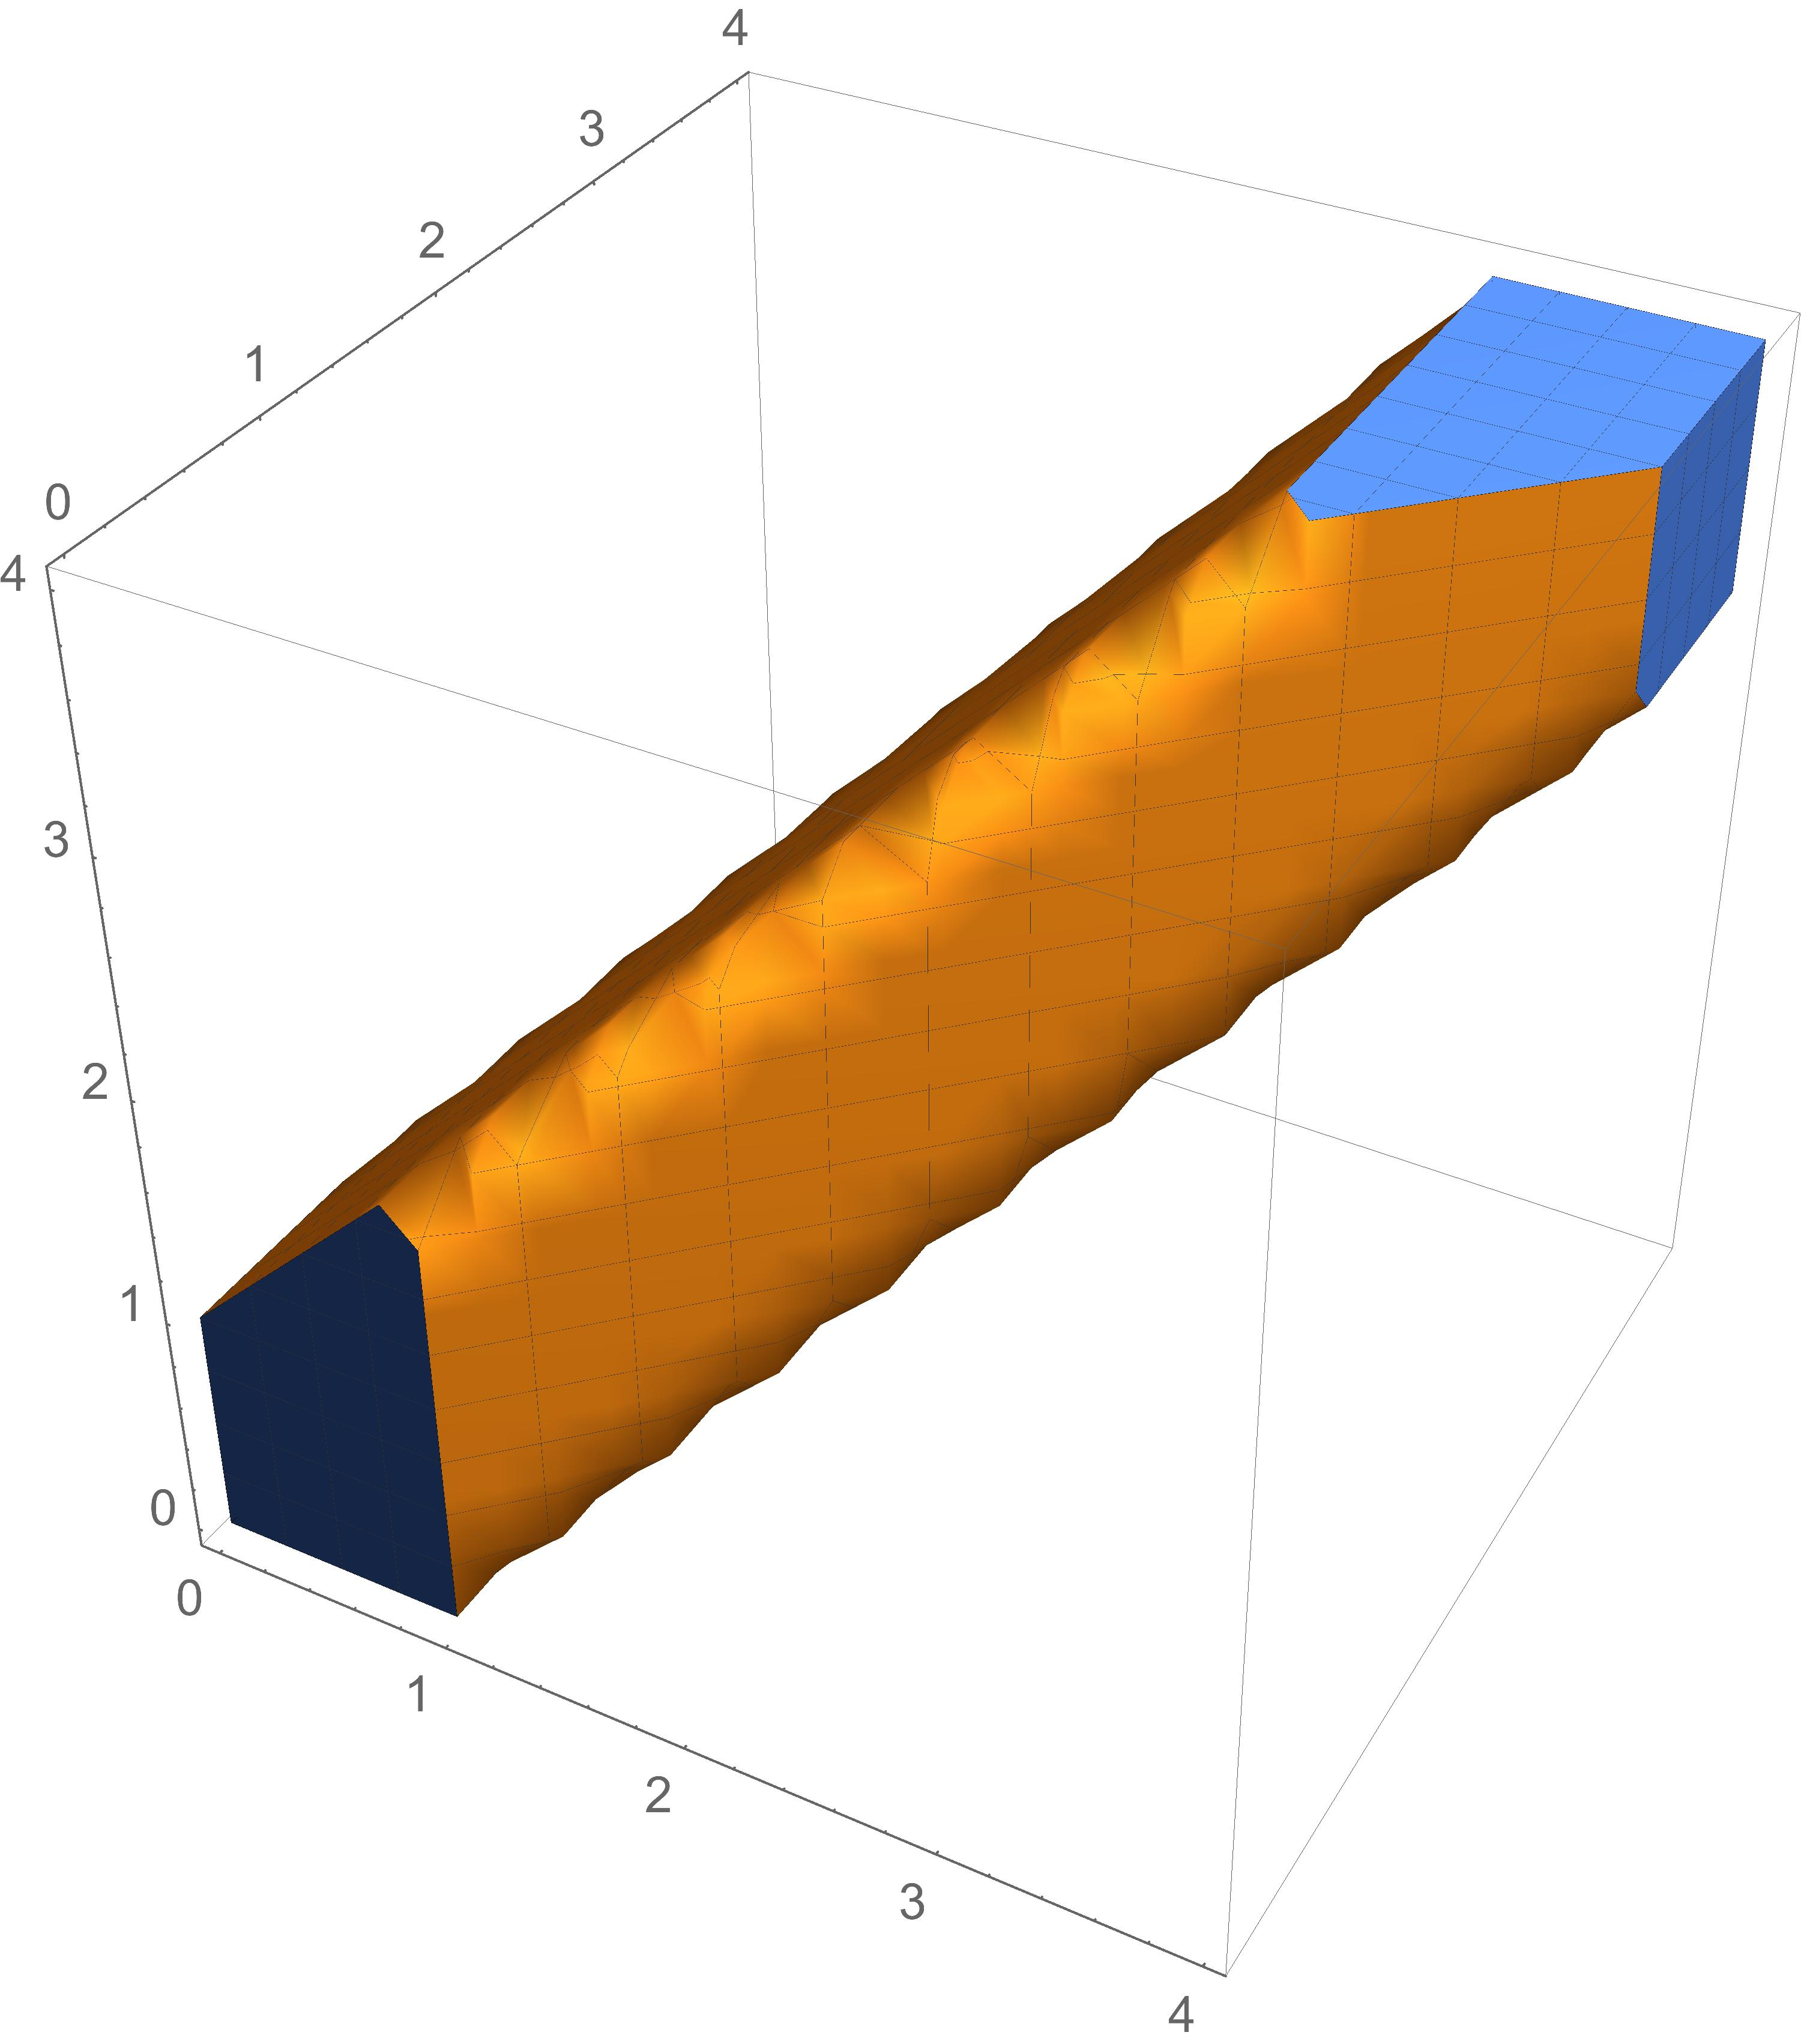
\includegraphics[scale=.6]{exercise8.jpg}
	\end{center}
\end{figure}
The above figure shows the feasible region. It is clearly closed (because of the inclusive inequalities) and and unbounded. However, the optimizer is at $(0,0,0)$ with an optimum of value, since the objective function is decreasing in each variable.

\subsubsection*{Exercise 8.9}
Consider the following linear program:
\begin{align*}
&\text{maximize} \ \ x + y + z \\
  &\text{subject to} \ \ -x + y \leq 1 \\
  &\qquad \qquad \ \ \ x - y \leq 1 \\
  &\qquad \qquad \ \ \ x - z \leq 1 \\
  &\qquad \qquad \ \ \ -x + z \leq 1 \\
  &\qquad \qquad \ \ \ x, y ,z \geq 0
\end{align*}
The feasible region for this region is the same as above. However, the objective function is now increasing in each argument. Since the feasible region is unbounded, there is no maximizer.

\subsubsection*{Exercise 8.10}
Consider the following linear program:
\begin{align*}
&\text{maximize} \ \ x + y + z \\
  &\text{subject to} \ \ -x + y \leq -1 \\
  &\qquad \qquad \ \ \ x - y \leq -1 \\
  &\qquad \qquad \ \ \ x - z \leq -1 \\
  &\qquad \qquad \ \ \ -x + z \leq -1 \\
  &\qquad \qquad \ \ \ x, y ,z \geq 0
\end{align*}
This problem has an empty feasible region. Consider the first constraint: $-x + y \leq 1$ implies that $x - y \geq 1$. Thus, no $x$ and $y$ can satisfy both $-x + y \leq 1$  and $x - y \leq -1$.

\subsubsection*{Exercise 8.11}
We can add extra constraints to the example used above to bound the feasible region (and exclude the origin):
\begin{align*}
&\text{maximize} \ \ x + y + z \\
  &\text{subject to} \ \ -x + y \leq 1 \\
  &\qquad \qquad \ \ \ x - y \leq 1 \\
  &\qquad \qquad \ \ \ x - z \leq 1 \\
  &\qquad \qquad \ \ \ -x + z \leq 1 \\
  &\qquad \qquad \ \ \ - x - y - z \leq -1 \\
  &\qquad \qquad \ \ \ x + y + z \leq 5 \\
  &\qquad \qquad \ \ \ x, y ,z \geq 0
\end{align*}
The feasible region is:
\begin{figure}[H]
  \centering
	\begin{center}
		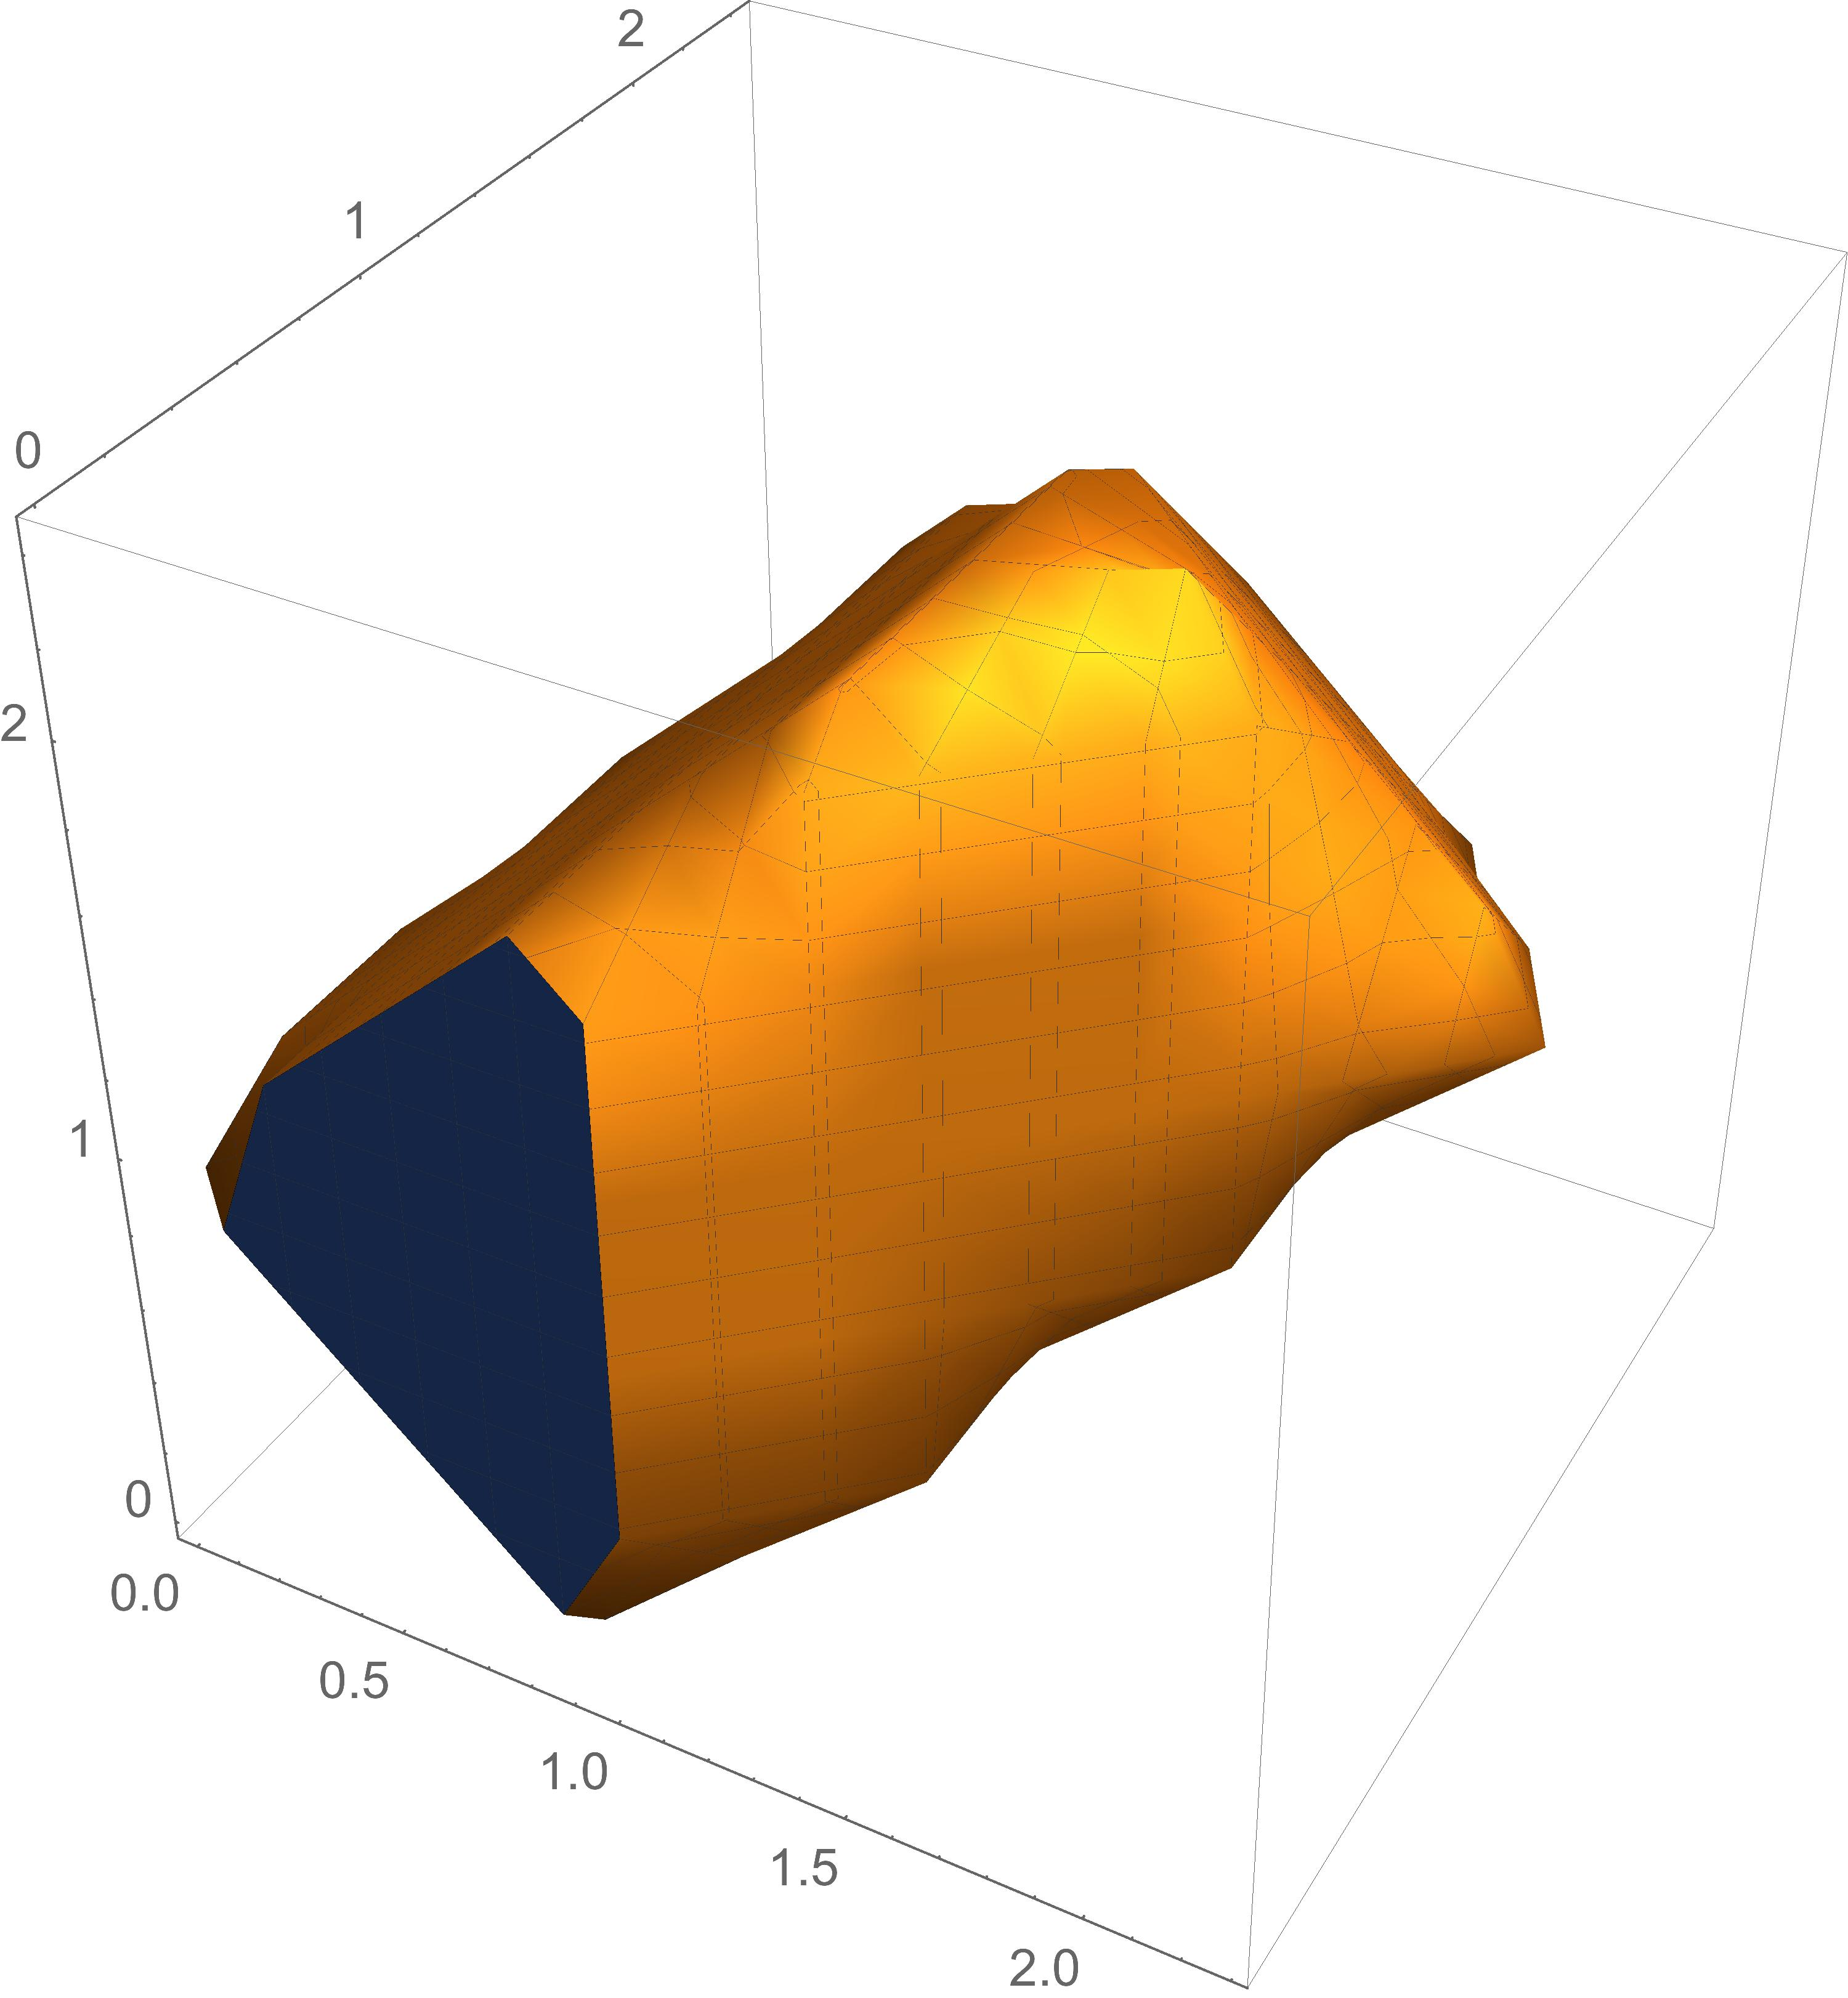
\includegraphics[scale=.6]{exercise11.jpg}
	\end{center}
\end{figure}
Thus, the feasible region is nonempty, closed, bounded, and the origin is not feasible. 
The auxillary problem is:
\begin{align*}
&\text{maximize} \ \ -x_0 \\
  &\text{subject to} \ \ -x + y + x_0 \leq 1 \\
  &\qquad \qquad \ \ \ x - y + x_0\leq 1 \\
  &\qquad \qquad \ \ \ x - z + x_0 \leq 1 \\
  &\qquad \qquad \ \ \ -x + z + x_0\leq 1 \\
  &\qquad \qquad \ \ \ - x - y - z + x_0 \leq -1 \\
  &\qquad \qquad \ \ \ x + y + z + x_0 \leq 5 \\
  &\qquad \qquad \ \ \ x, y ,z \geq 0
\end{align*}
The solution of this auxillary problem gives a feasible vertex for starting the original problem. We can see that "shifting" the original problem gives a feasible vertex for starting the simplex algorithm. 

\subsection*{Exercise 8.15}
\begin{claim}
	If $x \in \mathbb{R}^n$ is feasible for the primal and $y \in \mathbb{R}^m$ is feasible for the dual, then $c^Tx \leq b^Ty$. 
\end{claim}

\begin{proof}
	Let $x \in \mathbb{R}^n$ be feasible for the primal and $y \in \mathbb{R}^m$ be feasible for the dual. Therefore, $Ax \preceq b$ and $A^Ty \succeq b$. From these two relations, it follows that$(Ax)^T y \leq b^T y$ and $x^TA^Ty \geq x^Tc$. Thus,
	\begin{align*}
	c^T x &= x^T c \tag{since the dot product is scalar} \\
	&\leq x^TA^T y \\
	&= (Ax)^T y \\
	&\leq b^T y
	\end{align*}
\end{proof}

\subsection*{Exercise 8.17}
\begin{claim}
	For a linear optimization problem in standard form, the dual of the dual optimization problem is again the primal problem. 
\end{claim}
\begin{proof}
	Let a linear optimization problem in standard form be as follows:
	\begin{align*}
	\max_x \quad
	c^T x& \\
	\text{s.t.} \quad
	Ax &\preceq b \\
	x &\succeq 0
	\end{align*}
	and the dual problem is,
	\begin{align*}
	\min_y \quad
	b^T y& \\
	\text{s.t.} \quad
	A^Ty &\succeq c \\
	y &\succeq 0
	\end{align*}
	We can write the dual problem in standard form as follows:
	\begin{align*}
	\max_y \quad
	-b^T y& \\
	\text{s.t.} \quad
	-A^Ty &\preceq -c \\
	y &\succeq 0
	\end{align*}
	Then, the dual of this problem is,
	\begin{align*}
	\min_x \quad
	-c^T x& \\
	\text{s.t.} \quad
	(-A^T)^Tx &\succeq -b \\
	x &\succeq 0
	\end{align*}
	which is equivalent to,
	\begin{align*}
	\max_x \quad
	c^T x& \\
	\text{s.t.} \quad
	Ax &\preceq b \\
	x &\succeq 0
	\end{align*}
	which is simply the primal problem. 
\end{proof}

\subsection*{Exercise 8.18}
The dictionaries after each pivot of the primal problem are,
\begin{equation*}
\begin{matrix}
\zeta &= & & & x_1 &+& x_2 \\
\hline
w_1 &= &3 &-& 2x_1 &-& x_2\\
w_2 &= &5 &-& x_1 &-& 3x_2 \\
w_3 &= &4 &- & 2x_1 &-& 3x_2
\end{matrix}
\end{equation*}

\begin{equation*}
\begin{matrix}
\zeta &= &\frac{3}{2}&+& \frac{1}{2} x_2 &-& \frac{1}{2} w_1 \\
\hline
x_1 &= &\frac{3}{2} &-& \frac{1}{2} x_2 &-&\frac{1}{2} w_1\\
w_2 &= &\frac{7}{2}&-& \frac{5}{2} x_2 &+& \frac{1}{2} w_1 \\
w_3 &= &1 &- & 2x_2 &+& w_1
\end{matrix}
\end{equation*}

\begin{equation*}
\begin{matrix}
\zeta &= &\frac{7}{4}&-& \frac{1}{4} w_1 &-& \frac{1}{4} w_3 \\
\hline
x_1 &= &\frac{5}{4} &-& \frac{3}{4} w_1 &+&\frac{1}{4} w_3\\
w_2 &= &\frac{9}{4}&-& \frac{3}{4} w_1 &+& \frac{5}{4} w_3 \\
x_2 &= &\frac{1}{2} &+& \frac{1}{2} w_1 &-& \frac{1}{2} w_3
\end{matrix}
\end{equation*}
Thus, the optimizer is $(\frac{5}{4}, \frac{1}{2})$ and the optimum is $\frac{7}{4}$.

The dual of the linear problem is,
\begin{align*}
  \min_y\quad        &3y_1 + 5y_2 + 4y_3                    \\
  \text{s.t.\quad} & 2y_1 + y_2 + 2y_3 \geq 1 &    \\
                   & y_1 + 3y_2 + 3y_3 \geq 1      \\
                   & y_1, y_2 \geq 0          \\
\end{align*}
To use the simplex algorithm we need to write the dual problem in standard form: 
\begin{align*}
  \max_y\quad        &-3y_1 - 5y_2 - 4y_3                    \\
  \text{s.t.\quad} & -2y_1 - y_2 - 2y_3 \leq -1 &    \\
                   & -y_1 - 3y_2 - 3y_3 \leq -1      \\
                   & y_1, y_2 \geq 0          \\
\end{align*}
We first setup the auxiliary problem. The dictionaries after each pivot are:
\begin{equation*}
\begin{matrix}
\zeta &= & & & & & & & &-& x_0 \\
\hline
y_4 &=&-1 &+& 2y_1 &+& y_2 &+& 2y_3 &+& x_0  \\
y_5 &=&-1 &+& y_1 &+&3y_2 &+&3y_3&+& x_0
\end{matrix}
\end{equation*}

\begin{equation*}
\begin{matrix}
\zeta &=&-1&+&2y_1&+&y_2&+&2y_3&-&y_4 \\
\hline
x_0 &=&1 &-& 2y_1 &-& y_2 &-& 2y_3 &+& y_4  \\
y_5 &=& &-& y_1 &+&2y_2 &+&y_3&+& y_4
\end{matrix}
\end{equation*}

\begin{equation*}
\begin{matrix}
\zeta &= & & & & & & & &-& x_0 \\
\hline
y_2 &=&1 &-& 2y_1 &-& 2y_3 &+& y_4 &-& x_0  \\
y_5 &=&2&-&5y_1 &-&3y_3 &+&3y_4&-& 2x_0
\end{matrix}
\end{equation*}

Now, we continue with the original problem:
\begin{equation*}
\begin{matrix}
\zeta &=&-2&+&y_1&-&3y_2&-&2y_4 \\
\hline
y_3 &=&\frac{1}{2} &-& y_1 &-& \frac{1}{2} y_2 &+& \frac{1}{2}y_4  \\
y_5 &=&\frac{1}{2} &-&2y_1 &+&\frac{3}{2} y_2 &+&\frac{3}{2} y_4
\end{matrix}
\end{equation*}

\begin{equation*}
\begin{matrix}
\zeta &=&-\frac{7}{4}&-&\frac{9}{4} y_2&-&\frac{5}{4} y_4&-&\frac{1}{2} y_5 \\
\hline
y_1 &=&\frac{1}{4} &+&\frac{3}{4} y_2 &+&\frac{3}{4} y_4 &-&\frac{1}{2} y_5 \\
y_3 &=&\frac{1}{4} &-& \frac{5}{4} y_2 &-& \frac{1}{4} y_4 &+& \frac{1}{2}y_5  \\
\end{matrix}
\end{equation*}
Therefore, the optimizer is $(\frac{1}{4}, 0, \frac{1}{4})$ and the optimum is $\frac{7}{4}$.  Thus, the optimal values of the primal and dual problems are equal. 

\end{document}